\subsection{Methods}
% -------------------------------------------------------------------------
This section outlines the methods for performing the two types of
experiments presented in this work, developing
the procedures to automatically detect the solidifying melt pools as they
are observed, and the process for manually identifying the melt pools.
The presented procedures are written in the Python programming language
and formatted into \textit{Jupyter} notebooks \cite{jupyter}. Using Python
with \textit{Jupyter}
notebooks is beneficial for both development and presentation. The
cell-based nature of \textit{Jupyter} notebook files allow for an iterative
workflow for processing and analyzing data while also creating a
reproducible procedure in the process.
Variables declared in each cell are available to successive cells, allowing
for use of the same variables across a notebook, while showing the output of
a cell at any point of the procedure rather than at the end only.
Since cells can contain formatted text in
addition to code, scientific context can be provided about in addition to
technical information about the procedure itself in
between code cells, improving readability and reproducibility.
Other Python packages used in these procedures are
\textit{imageio} for reading and writing of image files \cite{imageio},
\textit{NumPy} for representing the images as numerical arrays and
performing fast calculations \cite{numpy}, \textit{scikit-image} for
performing image processing algorithms \cite{skimage}, and \textit{napari}
for visualizing and annotating the data with an interactive,
multi-dimensional image viewer \cite{napari}.

% -------------------------------------------------------------------------
\subsubsection{Ni-Mo-Al Simulated AM}
% -------------------------------------------------------------------------
Experiments simulating the processing conditions of LPBF were
performed using the AM simulator at sector 32-ID-B at the APS.
The simulator consists of an argon-backfilled chamber containing
a sample fixture holding a thin metallic plate sample
(approximately 100 µm thick) sandwiched between
two glassy carbon plates in the path of a polychromatic x-ray beam.
A 520 W laser is located above the sample. The
experiments are performed by striking the top surface of the metallic
sample with the laser, creating a pool of molten metal at the surface.
High-speed x-radiography captures the melting and solidification of the
sample with a downstream, high-speed detector. An image sequence through
time is captured with a spatial resolution of 1.93 µm
per pixel, a framerate of 80,000 frames per second, and a field-of-view of
988 by 741 µm. After the laser shuts off, the melted portion of the sample
(hereafter referred to as the melt pool) can be seen solidifying based on
the density and x-ray absorption differences between the liquid and the
solid phases (\ref{fig/rad-seq}).

\begin{figure}[ht!]
    \centering
    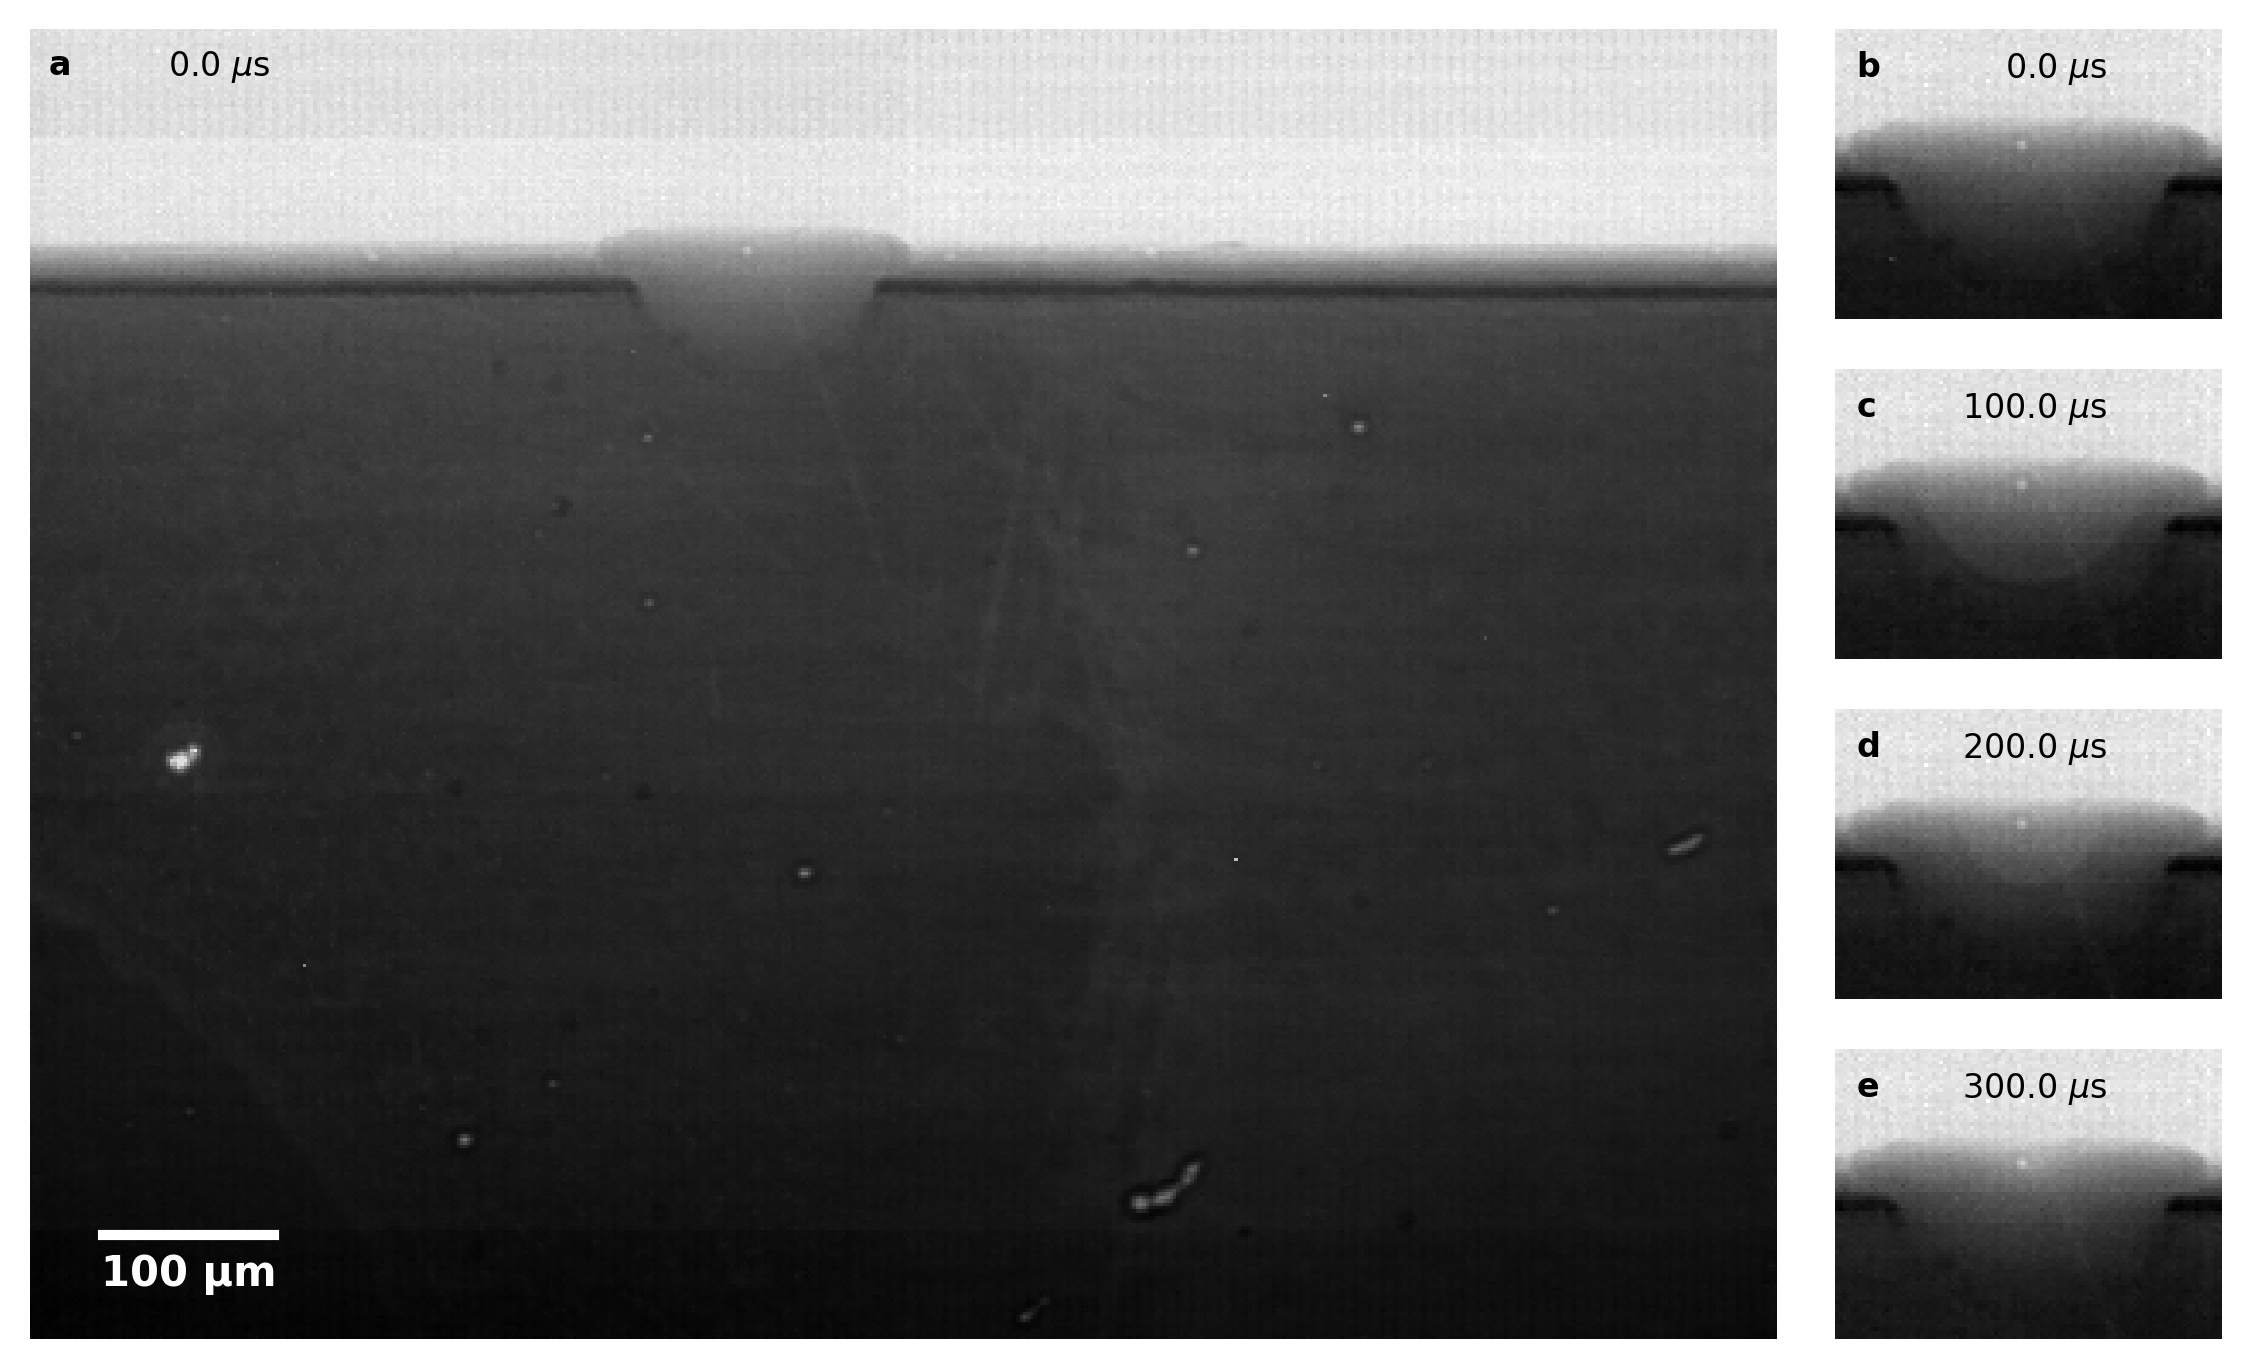
\includegraphics[width=0.75\textwidth]{figures/04/01-rad-seq.png}
    \caption{
        \small\setstretch{1}
        Subset of a time sequence of x-radiography depicting the solidification
        of a Ni-1.9 Mo-6.6 Al (wt.\%) single crystal after melting with a
        laser at 104 W (20\% maximum power).
        (a) Full image of radiograph right after the laser shuts off
        (t = 0 µs).
        (b) Radiograph from (a) cropped to the melt pool and immediate
        surroundings (t = 0 µs).
        (c) Cropped radiograph showing partial solidification and visible
        solid-liquid (S-L) interface (t = 100 µs).
        (d) Cropped radiograph showing further solidification and a smaller
        S-L interface (t = 200 µs).
        (e) Cropped radiograph showing near total solidification with S-L
        interface no longer easily visible (t = 300 µs).
    }
    \label{fig/rad-seq}
\end{figure}

\subsubsection{Simulated AM Detection Procedure}
% -------------------------------------------------------------------------
To measure solidification velocities during the AM-like process, the S-L
interface must be tracked through the radiograph sequence from the
experiment. Once the location is known, the change in location over time
yields the solidification velocity. To procedurally identify the S-L
interface, the images are processed in a way that highlights the
differences between each image and the preceding image in the time
sequence. The first step performed is the conversion of all images from
16-bit unsigned integer format to a floating-point image format
(\ref{fig/routine}.a). This changes the intensity range from
[0, 65536] to [0, 1] to enable floating point calculation and prevent a loss
of information from rounding to the nearest integer. Next, a
Gaussian filter is applied to each image. This smooths out noise in
the images. Each smoothed image is then subtracted from the succeeding
image (\ref{fig/routine}.b). The resulting subtracted image visually
highlights the moving
interface and some varying noise in the images, since it is these features
that are the areas of greatest difference in the sequence. The intensity
of the subtracted image is rescaled by clipping the intensity of the
image. This replaces the pixels with intensities in the upper and lower
fifth percentile with the intensity value at those cutoffs
respectively (\ref{fig/routine}.c).
The rescaled images are denoised using a total
variation minimization algorithm \cite{Kokaram2004} implemented in
\textit{scikit-image} as the function
\textit{restoration.denoise\textunderscore tv\textunderscore chambolle}.
This further reduces the intensity of the remaining noisy regions in
the image. The image is inverted so the regions
corresponding to the S-L interface region are represented by high
intensities in the image (\ref{fig/routine}.d). An upper minimum
threshold is applied to the inverted image to create a binary image
(\ref{fig/routine}.e). A skeletonization algorithm \cite{Zhang1984}
implemented in scikit-image as the function \textit{morphology.skeletonize}
is used to erode each connected region in the image to one-pixel wide
``skeleton'' regions in the binary image (\ref{fig/routine}.f).

\begin{figure}[ht!]
    \centering
    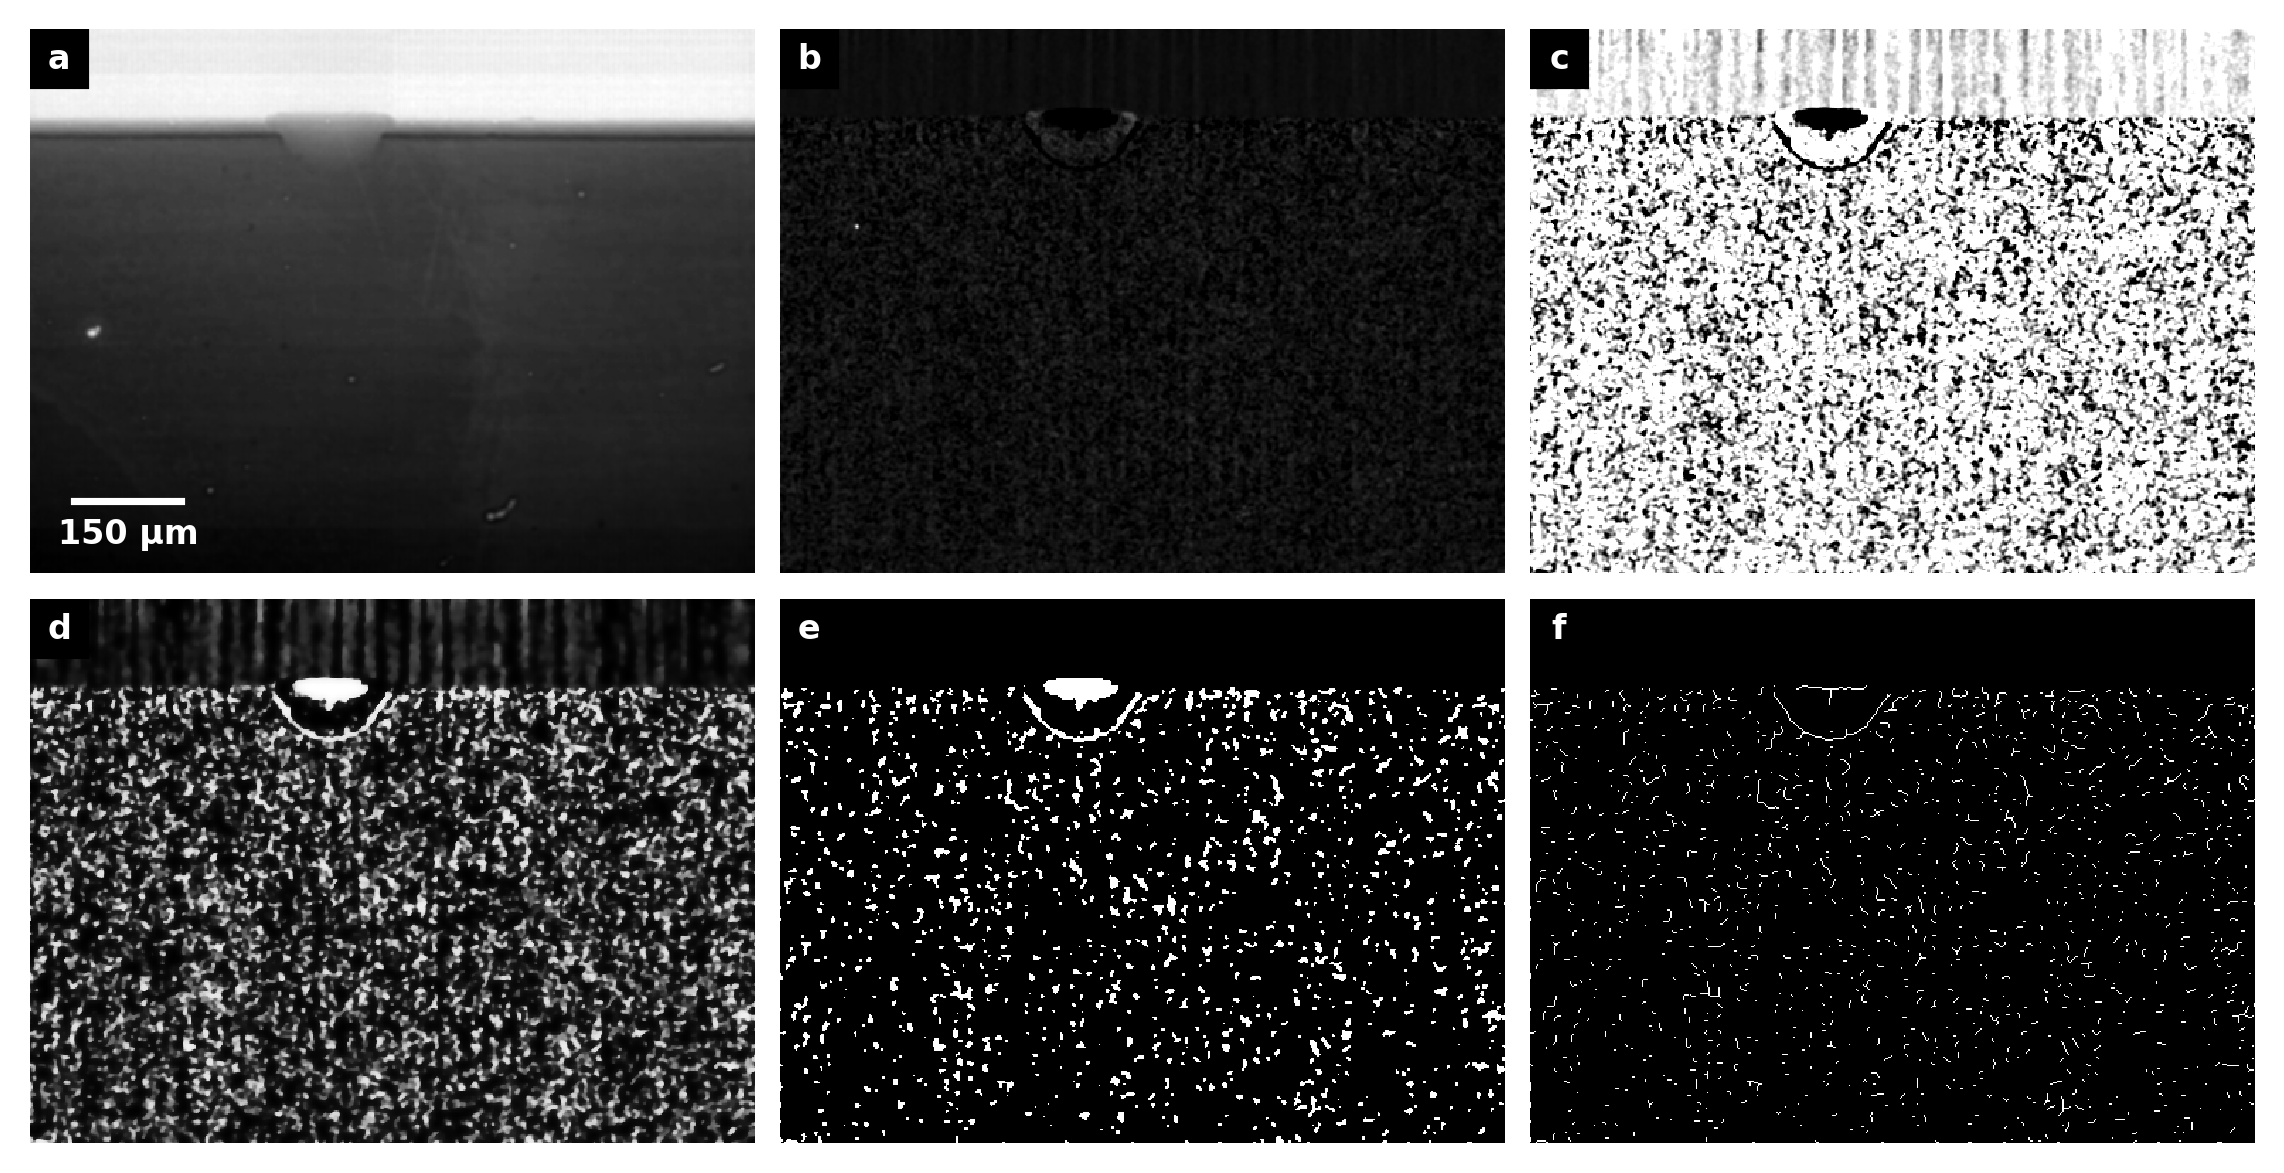
\includegraphics[width=0.75\textwidth]
    {figures/04/02-routine.png}
    \caption{
        \small\setstretch{1}
        The procedural image processing routine for identifying the
        solid-liquid (S-L) interface for a radiograph taken during the
        solidification portion of the experiment.
        (a) Raw radiograph showing the melt pool and S-L interface.
        (b) Smoothing with a Gaussian filter and subtraction from the
        succeeding smoothed radiograph in the time sequence.
        (c) Intensity rescaling by clipping the top and bottom five percent
        intensities.
        (d) Denoising and intensity inversion.
        (e) Upper minimum threshold to convert to binary image.
        (f) Skeletonization to create one-pixel wide regions.
    }
    \label{fig/routine}
\end{figure}

The area of each skeleton region is analyzed using the function
\textit{measure.regionprops} from \textit{scikit-image}.
Since each region is one pixel
wide, the area corresponds to the total length of the skeleton with each
separate branch or ``bone'' laid end-to-end. For most images in the
sequence, the largest skeleton correlates to the S-L interface. This is
seen by overlaying the largest skeleton over the solidifying melt pool
radiographs within the first 200 µs after the laser shuts off
(\ref{fig/skel-overlay}).

\begin{figure}[ht]
    \centering
    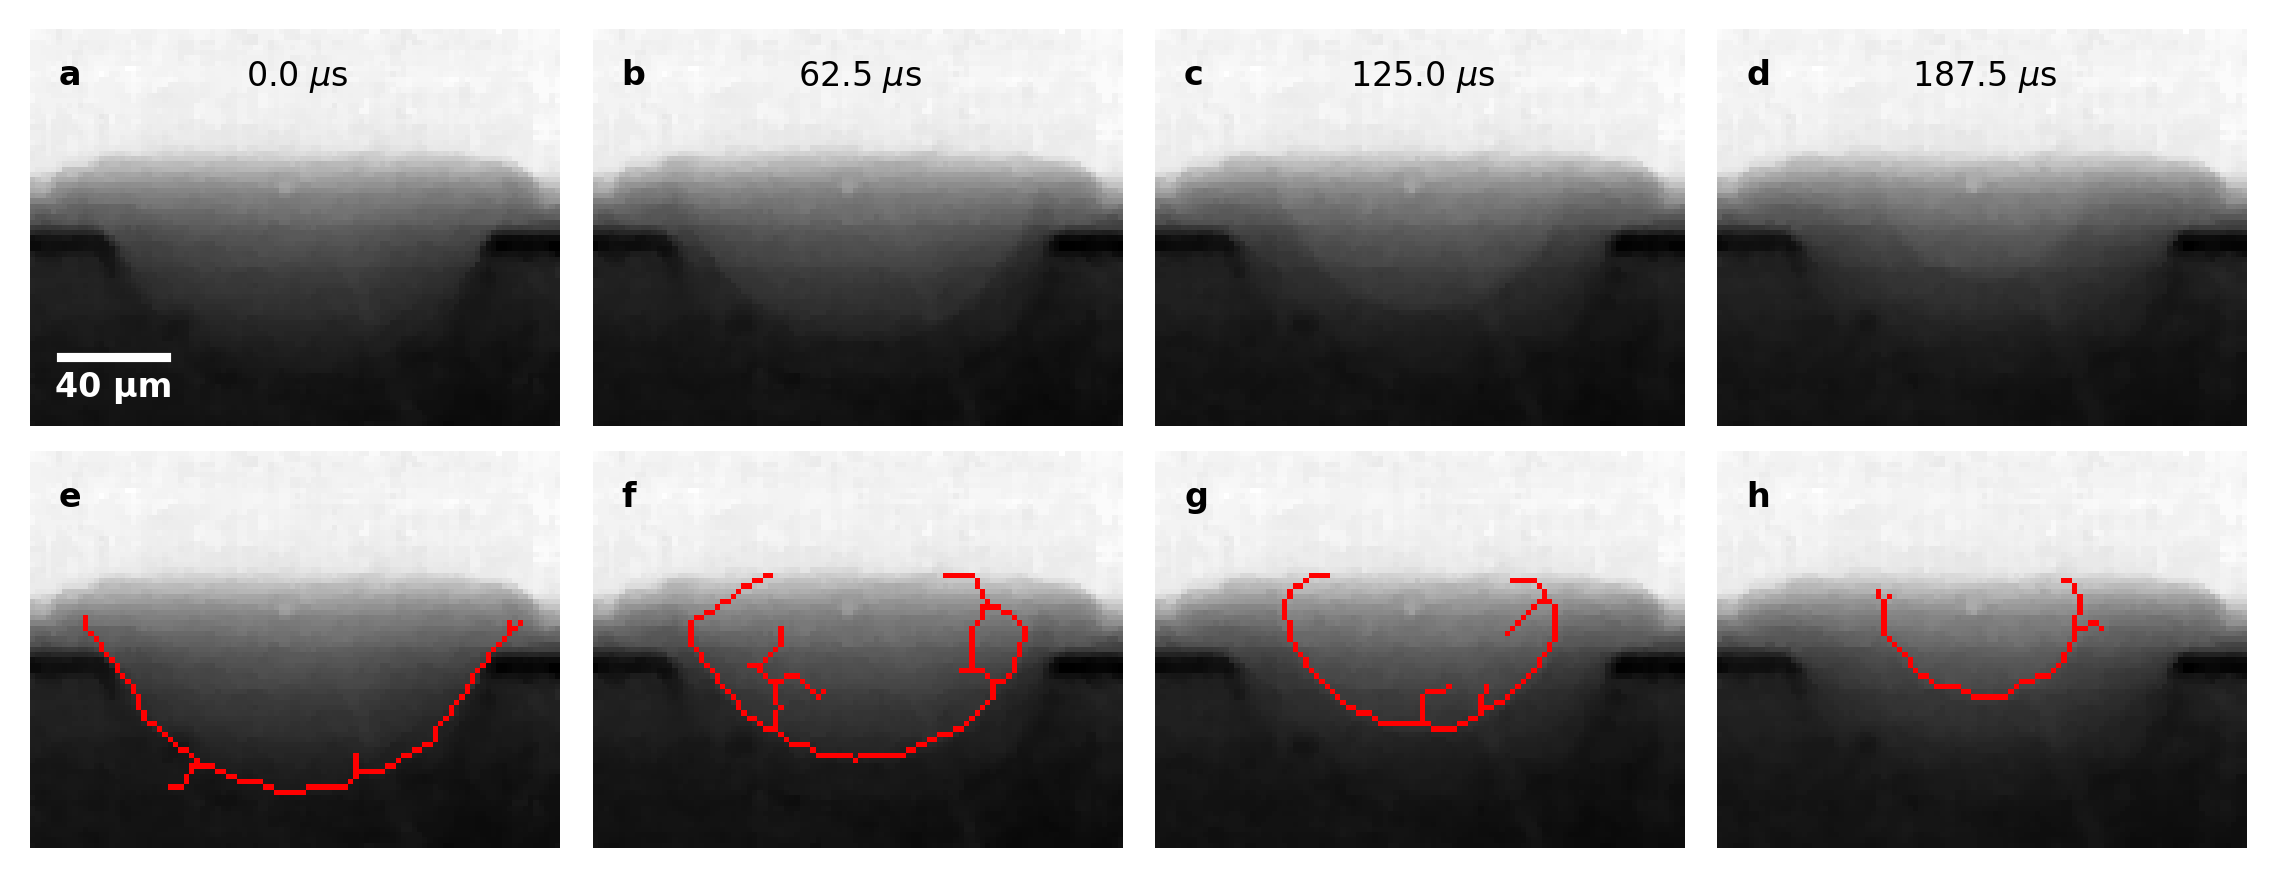
\includegraphics[width=0.9\textwidth]{figures/04/03-skel-overlay.png}
    \caption{
        \small\setstretch{1}
        (a - d) Subset of radiography sequence, showing the solid-liquid
        interface receding throughout the experiment.
        (e - f) Skeletonized regions overlaid in red on subset of
        radiography sequence, showing the as-detected position of the
        solid-liquid interface throughout the experiment.
    }
    \label{fig/skel-overlay}
\end{figure}

\subsubsection{Simulated AM Manual Measurements}
% -------------------------------------------------------------------------
The position of the detected S-L interfaces was compared to manual
measurements to assess the performance of the detection procedure.
The Python package \textit{napari} enables a graphic user interface (GUI)
window to annotate multi-dimensional images, which was used to manually
track the interfaces. The sequence of radiographs was opened in a
\textit{napari} series of frames segmented from the raw image.
A \textit{napari} points layer was also added to the window. This allowed a
user to annotate the images with a point denoting the bottom of the interface
for each image. This manual annotation was performed three times such that
the variance of individual manual measurements could be analyzed and
compared to the mean manual measurement along with the detected S-L
interface locations.

